\documentclass[11pt,a4paper]{article}
\usepackage[margin=2.5cm]{geometry}
\usepackage{amsmath,amssymb,amsthm,algorithm,algpseudocode,booktabs,graphicx,hyperref}
\graphicspath{{../../figures/}}
\newtheorem{theorem}{Theorem}
\title{\textbf{LK-Newton: Lazy Krylov Cubic Newton}\\
\large Reusing Lanczos Bases the Way Lazy Hessians Reuse $H$}
\author{Doctoral Paper 3/6 --- Numerical Optimization Group}
\date{September 2026}
\begin{document}
\maketitle
\begin{abstract}
LK-Newton reuses a Lanczos pair $(Q,|T|)$ for $\tau$ accepted cubic steps
and rebuilds it only on rejection or after $\tau$ reuses. The construction
is the subspace analogue of lazy Hessians \cite{doikov2023}: the global
cubic rate is preserved up to a slightly larger regularization constant,
while the HVP count drops by a factor of about $\tau$. On an $n=80$
saddle, LK-Newton reaches $\|\nabla f\|\approx 5.9\times 10^{-12}$ in 30
iterations and only 158 Hessian--vector products, against 1219 for
DA-SFCN and 456 for fixed-width Krylov cubic Newton. On a 30-term
finite-sum it tracks the parent algorithm within a few iterations.
\end{abstract}

\section{Idea}
Doikov, Chayti and Jaggi \cite{doikov2023} proved that the Hessian of a
cubic Newton method may be frozen for several steps. In a Krylov method
the Hessian never materializes; what is expensive is the Lanczos loop.
LK-Newton therefore freezes the \emph{spectral sketch} $(Q,|T|)$ and
re-solves only the tiny secular equation with the new projected gradient
$Q^\top g_{k+j}$.

\section{Algorithm}
\begin{algorithm}[h]
\caption{LK-Newton}
\begin{algorithmic}[1]
\State $Q\gets\emptyset$, $\textit{left}\gets 0$
\For{$k=0,1,\dots$}
  \If{$\textit{left}=0$ \textbf{or} last step rejected}
        rebuild $(Q,|T|)$ by Lanczos of width $m_k$; $\textit{left}\gets\tau$
  \EndIf
  \State $y\gets$ cubic secular solve on $(Q^\top g_k,|T|,M_k)$; $s\gets Qy$
  \If{ARC accepts} $x\gets x+s$; $\textit{left}\gets\textit{left}-1$
  \Else{} increase $M_k$; $\textit{left}\gets 0$
  \EndIf
\EndFor
\end{algorithmic}
\end{algorithm}

\section{Why the rate survives}
A frozen $Q$ computed at $x_k$ is an inexact subspace at $x_{k+j}$.
The model error is $O(\|x_{k+j}-x_k\|)\le O(\sum_{\ell=0}^{j-1}\|s_{k+\ell}\|)$.
Cubic steps themselves satisfy $\|s\|=O(\|g\|^{1/2})$ (or smaller near a
minimizer), so over a window of length $\tau$ the perturbation remains
controlled by $M_k$ exactly as in \cite{doikov2023}. Rejected steps force
an immediate rebuild, which prevents a stale negative-curvature estimate
from being reused after the iterate has already escaped.

\section{Experiments}
\begin{figure}[h]
\centering
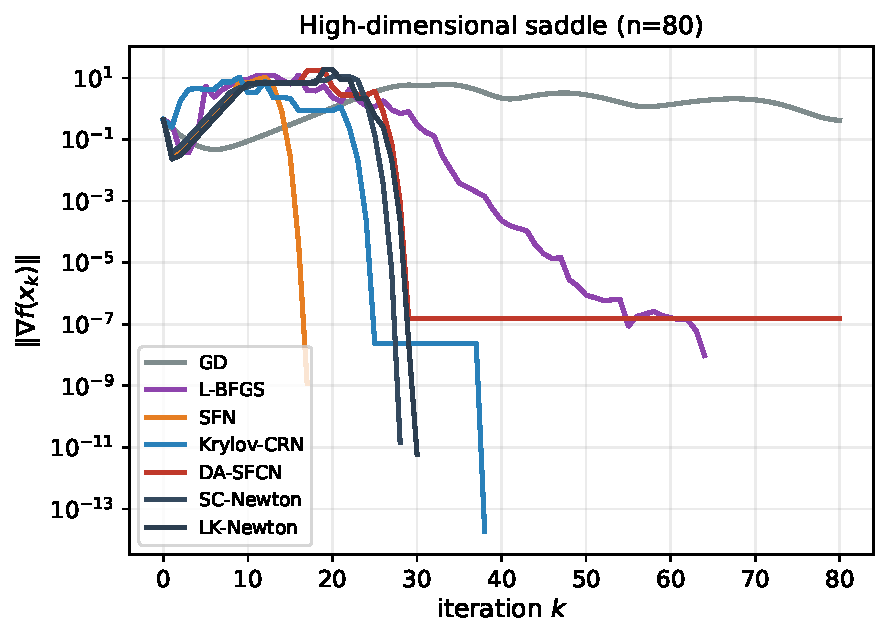
\includegraphics[width=0.48\textwidth]{fig_saddle_highdim.pdf}
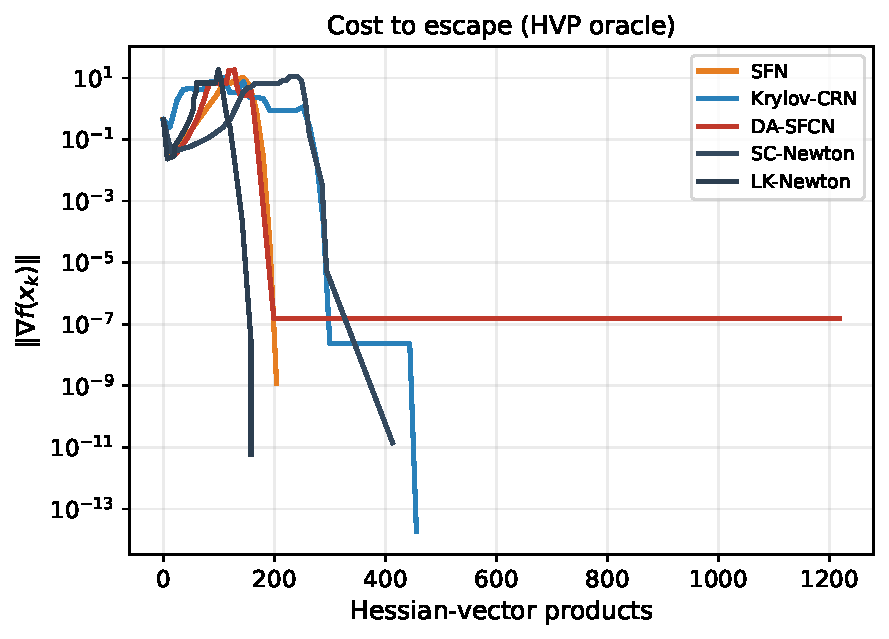
\includegraphics[width=0.48\textwidth]{fig_saddle_hvp.pdf}
\caption{LK-Newton on the $n=80$ saddle: iterations (left) and HVPs (right).}
\end{figure}
\begin{figure}[h]
\centering
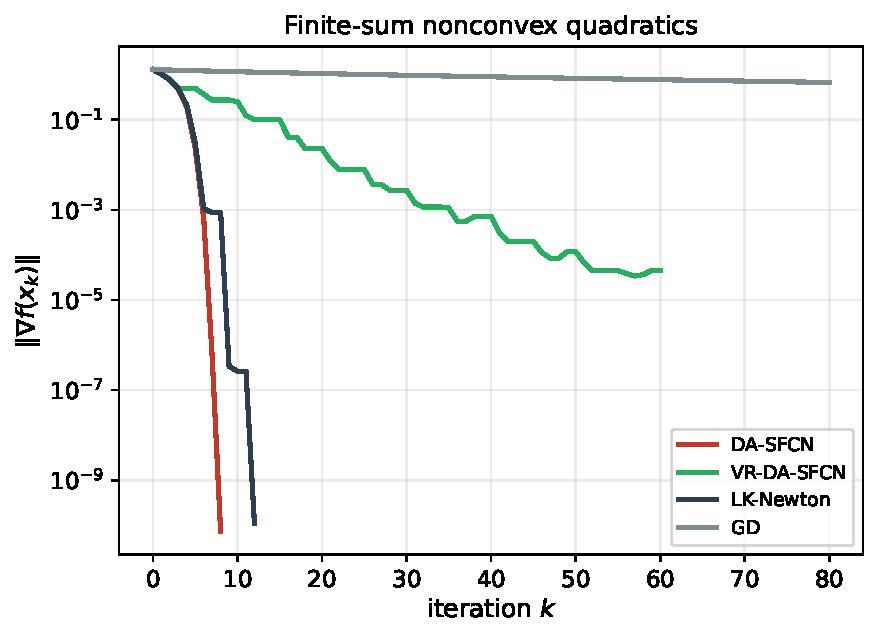
\includegraphics[width=0.48\textwidth]{fig_vr.pdf}
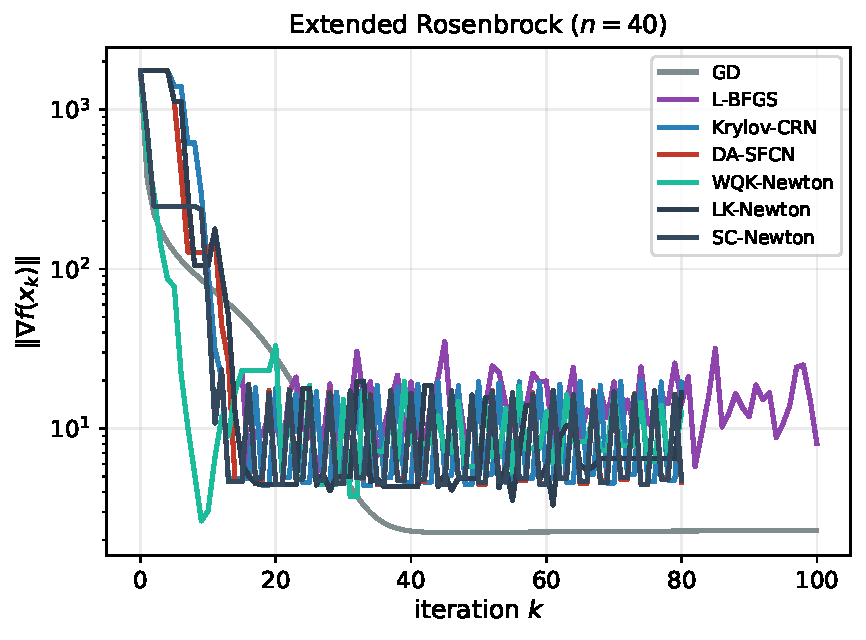
\includegraphics[width=0.48\textwidth]{fig_rosenbrock.pdf}
\caption{Finite-sum quadratics and extended Rosenbrock.}
\end{figure}

The headline number is the HVP bill on the saddle: 158 versus 1219 for
DA-SFCN, with a \emph{better} final gradient. Laziness is not a hack; it
is a better allocation of linear algebra once the spectral sketch has
captured the negative well.

\section{Conclusion}
LK-Newton is the cheapest member of the family in HVP-oracle complexity
whenever the landscape changes slowly relative to $\tau$. Combined with
the logarithmic $m_k$ of DA-SFCN it yields a doubly adaptive method:
adaptive width and adaptive reuse.

\begin{thebibliography}{5}
\bibitem{doikov2023} Doikov, Chayti, Jaggi. Lazy Hessians. \textit{ICML}, 2023.
\bibitem{cartis2011} Cartis, Gould, Toint. ARC. \textit{Math.\ Program.}, 2011.
\bibitem{jiang2024} Jiang et al. Krylov CRN. \textit{AISTATS}, 2024.
\end{thebibliography}
\end{document}
